\section{Residual Neural Networks}
\label{sec:neural-networks}

What I want to write here/ goal of this section:
\begin{itemize}
	\item Explain how ResNets work
	\item Explain why they are used / what problem they solve
	\item Show some applications
	\item Show some examples of Block Design
	\item Los gehts!
\end{itemize}

In the early 2010s, when neural networks started to become increasingly popular it was still difficult to train models with many layers.
Neural network architectures with many layers ("deep" networks) have led to many breakthroughs in supervised learning tasks.
There is evidence that the number of layers (the depth) is of high importance:
Non-flattening theorems state the the number of neurons required by a shallow network, i.e. one with only one hidden layer, grows (almost) exponentially compared to a deep network \cite{lin17,delalleau11}.
An example: the product of $n$ numbers can be computed by a deep network with only $4n$ neurons, where as a flattened equivalent with only one hidden layer would require $2^n$ neurons \cite{lin17}.

These facts justify the conjecture that the deeper a network is, the better its performance.
The greater number of parameters resulting from added layers should lead to an improvement --  or at least not worsen the results.
\citet{he16} constructed an easy example for a deeper network with the same performance as a shallow one:
Take a trained (shallow) network and copy its parameters to the first layers of the deep network.
Set the remaining layers such that they perform an identity mapping, which means they just pass the input through to the next layer without changing it.
This indicates that in general, a deeper network should not produce worse results than one with fewer layers.

\begin{figure}
	\makebox[\textwidth][c]{
		\centering
		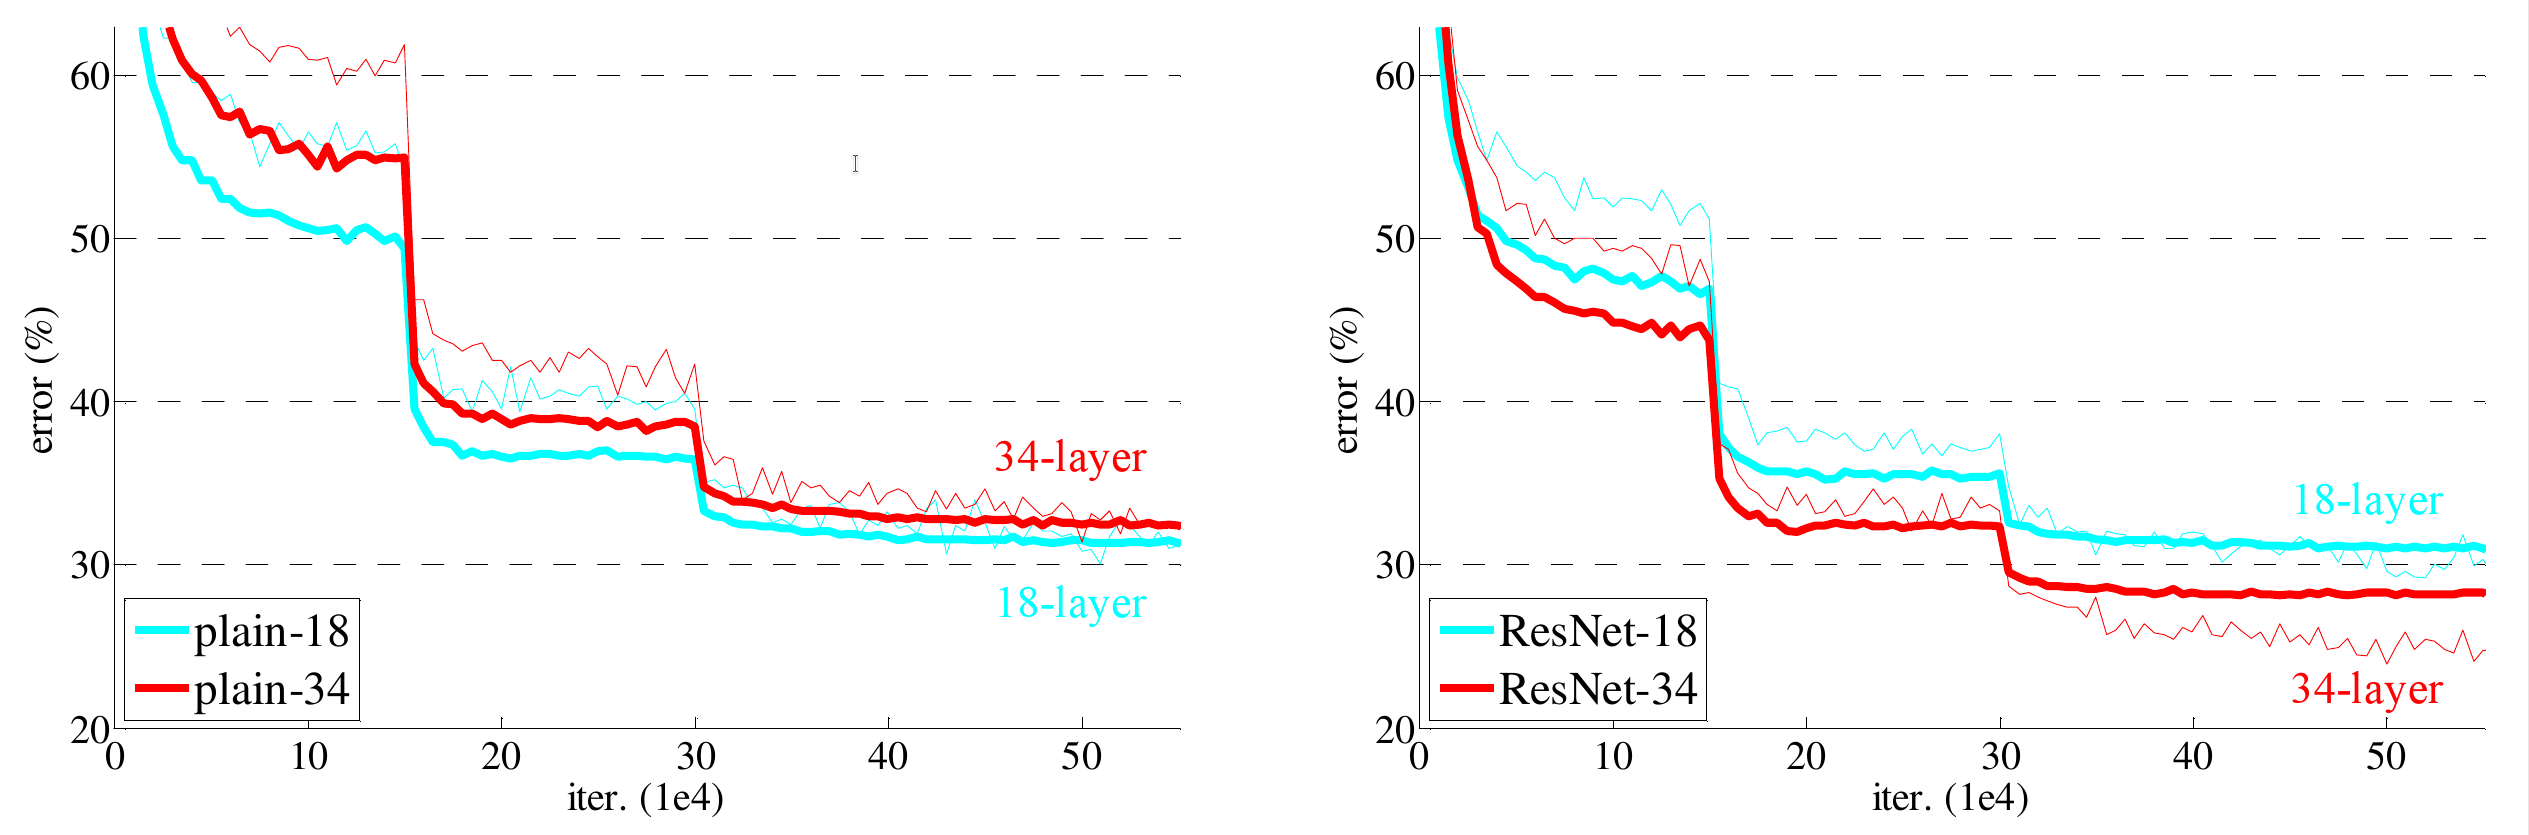
\includegraphics[scale=0.4]{figures/image_net_error_by_kaiming_he.png}
	}
	\caption{
		Training (thin) and validation errors (bold) for a 18- and 34-layer plain network (left) and ResNet (right).
		The plain 34 layer network shows worse results than the 18 layer equivalent, whereas the deeper ResNet performs better than the 18 layer one.
		This is not the case for the plain network.
		This figure originates from the paper "Deep Residual Learning for Image Recognition" by \citet{he16}. \copyright~2016 IEEE.}
	\label{fig:depth-performance-decline}
\end{figure}

Yet in practice one can observe deteriorating performance after a certain depth, which can be seen in \cref{fig:depth-performance-decline}.
This decline is measurable not only for the test error (which might indicate overfitting), but also for the training error.
It seems that contemporary optimizers are not able to effectively learn the solution constructed above.
Thus, \citet{he16} conjecture that it is hard to learn the identity mapping through non-linear layers and suggest that it is easier to learn the zero function instead.
This leads to their proposed network architecture: Residual Neural Networks (ResNets).

The characteristic feature of ResNets is that they learn residual mappings.
Let $f(x)$ be the desired mapping learned by a number of non-linear layers with input $x$.
Instead of learning $f(x)$ \citet{he16} suggest learning the function $g(x) \coloneqq f(x) - x$ -- the \emph{residual} -- instead.
This is implemented by creating shortcut connections that skip one or more layers and are add the input to the layers' output, resulting in $g(x) + x = f(x)$.
\cref{fig:residual-block}